% ============================================================
% Week 4 -- Normal equations
% ============================================================
\chapter{Least Squares and the Normal Equations}\label{ch:week04}

This chapter covers Week~4 (Lectures 11--14). The instructor's handwritten notes for this week
are divided into ``Lecture 2'', ``Lecture 3'' and ``Lecture 4''. We match them to the videos by
title: the normal equations (video 12), the uniqueness theorem (video 13), and the projection
and matrix review (video 14). The first part of the notes, which recalls the models and
classifications, goes with video 11.

% ============================================================
% Lecture 11 -- Different classifications of linear models
% ============================================================
\section{Different Classifications of Linear Models}\label{sec:L11}

\lectureheader{11}{pNIF__GOLGo}{Week-4 handwritten notes \texttt{Feb14.pdf}, first part (``Recall: linear model'', examples 1--3, exercise ``express 1, 2, 3 as $(Y,X\beta,\sigma^2I)$''); Week-5 assignment Q3}

\begin{guiding*}
By the end of this lecture you should be able to:
\begin{itemize}
  \item recall the linear model $(Y,X\beta,\sigma^2I_n)$ and its ingredients;
  \item write down explicitly the design matrices of the one-way, nested and two-way classification models;
  \item compute the rank of these design matrices and say how many linear combinations of the parameters can be estimated.
\end{itemize}
\end{guiding*}

\subsection{Recall: the linear model}
The data are $n$ observations $Y_1,\dots,Y_n$, and the parameters are $\beta_1,\dots,\beta_p$ (the
notes write $m$). The model is
\[
Y_i=\sum_{j=1}^p x_{ij}\beta_j+\eps_i,\qquad \EE[\eps_i]=0,\quad \Var(\eps_i)=\sigma^2,\quad \eps_i\text{ uncorrelated},
\]
or $Y=X\beta+\eps$ with $\EE[\eps]=0$ and $\Cov(\eps)=\sigma^2I_{n}$. We write it as
$(Y,X\beta,\sigma^2I_n)$: the data, their expectation, and their variance--covariance matrix
(\cref{def:L09-matrix}).

The three examples of \cref{sec:L09} are recalled:
\begin{enumerate}
  \item one-way classification: $Y_{ij}=\mu+\mu_i+\eps_{ij}$, $1\le j\le n_i$, $1\le i\le k$;
  \item nested classification: $Y_{ijl}=\mu+\mu_i+\delta_{ij}+\eps_{ijl}$, $1\le l\le n_{ij}$, $1\le j\le m_i$, $1\le i\le k$;
  \item two-way classification: $Y_{ijl}=\mu+\alpha_i+\beta_j+\gamma_{ij}+\eps_{ijl}$, $1\le l\le n_{ij}$, $1\le j\le J$, $1\le i\le I$.
\end{enumerate}
The exercise in the notes (also Week-5 assignment Q3) is to express each of them as
$(Y,X\beta,\sigma^2I_n)$. We do this in general and then for small cases.

\subsection{A general principle}
\begin{definition}[Indicator columns]\label{def:L11-indicator}
For a classification with observations labelled by cells, the \vocab{indicator column} of a
level (or cell) $c$ is the $0/1$ vector with a $1$ exactly in the rows of observations belonging
to $c$. In all three models, $X$ is obtained by listing the observations in a fixed order (say
lexicographic in $(i,j,l)$) and writing one column for each parameter: $\one_n$ for $\mu$, and the
indicator column of the corresponding level or cell for every other parameter.
\end{definition}
Indeed, the coefficient of a parameter in the equation for $Y_{ijl}$ is $1$ if the parameter
appears in that equation and $0$ otherwise.

\subsection{Model 1: one-way classification}
\begin{example}[$k=3$, $n_1=n_2=n_3=2$]\label{ex:L11-oneway}
$Y=(Y_{11},Y_{12},Y_{21},Y_{22},Y_{31},Y_{32})\T$ and $\beta=(\mu,\mu_1,\mu_2,\mu_3)\T$:
\[
X=\begin{pmatrix}
1&1&0&0\\1&1&0&0\\1&0&1&0\\1&0&1&0\\1&0&0&1\\1&0&0&1
\end{pmatrix},\qquad n=6,\ p=4,\ \rank X=3 .
\]
\end{example}
By \cref{prop:L08-rank}, $\rank X=k$ in general.

\subsection{Model 2: nested classification}
\begin{example}[$k=2$, $m_1=m_2=2$, $n_{ij}=2$]\label{ex:L11-nested}
$\beta=(\mu,\mu_1,\mu_2,\delta_{11},\delta_{12},\delta_{21},\delta_{22})\T$ and
$Y=(Y_{111},Y_{112},Y_{121},Y_{122},Y_{211},Y_{212},Y_{221},Y_{222})\T$:
\[
X=\begin{pmatrix}
1&1&0&1&0&0&0\\
1&1&0&1&0&0&0\\
1&1&0&0&1&0&0\\
1&1&0&0&1&0&0\\
1&0&1&0&0&1&0\\
1&0&1&0&0&1&0\\
1&0&1&0&0&0&1\\
1&0&1&0&0&0&1
\end{pmatrix},\qquad n=8,\ p=7,\ \rank X=4 .
\]
\end{example}

\begin{proposition}\label{prop:L11-nestedrank}
In the nested model with every $n_{ij}\ge1$, $\rank X=\sum_{i=1}^k m_i$, the number of subgroups.
\end{proposition}
\begin{proof}
Let $d_{ij}$ be the indicator column of subgroup $(i,j)$. These columns are non-zero and have
disjoint supports, so, as in the proof of \cref{prop:L08-rank}, they are linearly independent.
The remaining columns are sums of them: the column of $\mu_i$ is $\sum_{j=1}^{m_i}d_{ij}$ and the
column of $\mu$ is $\sum_{i,j}d_{ij}$. Hence $\colsp{X}=\mathrm{span}\{d_{ij}\}$, which has dimension $\sum_i m_i$.
\end{proof}

\subsection{Model 3: two-way classification}
\begin{example}[$I=J=2$, $n_{ij}=2$]\label{ex:L11-twoway}
$\beta=(\mu,\alpha_1,\alpha_2,\beta_1,\beta_2,\gamma_{11},\gamma_{12},\gamma_{21},\gamma_{22})\T$ and $Y$
ordered as $Y_{111},Y_{112},Y_{121},Y_{122},Y_{211},Y_{212},Y_{221},Y_{222}$:
\[
X=\begin{pmatrix}
1&1&0&1&0&1&0&0&0\\
1&1&0&1&0&1&0&0&0\\
1&1&0&0&1&0&1&0&0\\
1&1&0&0&1&0&1&0&0\\
1&0&1&1&0&0&0&1&0\\
1&0&1&1&0&0&0&1&0\\
1&0&1&0&1&0&0&0&1\\
1&0&1&0&1&0&0&0&1
\end{pmatrix},\qquad n=8,\ p=9,\ \rank X=4 .
\]
\end{example}

\begin{proposition}\label{prop:L11-tworank}
In the two-way model with interaction and every $n_{ij}\ge1$, $\rank X=IJ$, the number of cells.
In the \emph{additive} two-way model $Y_{ijl}=\mu+\alpha_i+\beta_j+\eps_{ijl}$ (no $\gamma_{ij}$), with every
$n_{ij}\ge 1$, $\rank X=I+J-1$.
\end{proposition}
\begin{proof}
With interaction: the $IJ$ cell indicators $g_{ij}$ (the columns of the $\gamma_{ij}$) are non-zero with disjoint
supports, so they are independent. The other columns are sums of them: $\alpha_i\mapsto\sum_j g_{ij}$,
$\beta_j\mapsto\sum_i g_{ij}$, $\mu\mapsto\sum_{i,j}g_{ij}$. So $\colsp{X}=\mathrm{span}\{g_{ij}\}$ has dimension $IJ$.

Additive model: the columns are $\one$, $a_i=\sum_j g_{ij}$ and $b_j=\sum_i g_{ij}$. Since
$\sum_i a_i=\sum_jb_j=\one$, the column space is spanned by $a_1,\dots,a_I,b_1,\dots,b_J$, and there is at least the one
relation $\sum a_i-\sum b_j=0$. So the rank is at most $I+J-1$. To see that it is exactly $I+J-1$, suppose
$\sum_i s_ia_i+\sum_j t_jb_j=0$. Every cell is non-empty, so reading the row of an observation in
cell $(i,j)$ gives $s_i+t_j=0$ for all $i,j$. Hence $s_i=-t_1$ for all $i$ and $t_j=-s_1$ for all $j$, so
all $s_i$ equal some $s$ and all $t_j=-s$. The relations form a $1$-dimensional space, so the
$I+J$ columns $a_i,b_j$ span a space of dimension $I+J-1$.
\end{proof}

\begin{note}[How many parameters can we estimate?]
The rank tells us how many linearly independent linear parametric functions are estimable
(\cref{cor:L10-subspace}): $k$ of the $k+1$ in Model~1, $\sum m_i$ of the $1+k+\sum m_i$ in Model~2,
and $IJ$ of the $1+I+J+IJ$ in Model~3. The estimable functions are exactly the combinations of
cell means. In the next lectures we find \emph{how} to estimate them: by least squares.
\end{note}

\begin{note}[Supplementary: Kronecker-product form]
With equal replication the design matrices have a compact form. In Model~1 with $n_i\equiv m$:
$X=[\one_k\otimes\one_m,\ I_k\otimes\one_m]$. In Model~3 with $n_{ij}\equiv m$:
$X=[\one_I\otimes\one_J\otimes\one_m,\ I_I\otimes\one_J\otimes\one_m,\ \one_I\otimes I_J\otimes\one_m,\ I_I\otimes I_J\otimes\one_m]$.
The notebook builds the matrices of this lecture both ways.
\end{note}

\subsection{Computation}
\nb{week04/L11\_classification\_designs.ipynb} writes a general function that builds the design
matrix from factor labels, checks the ranks of \cref{prop:L11-nestedrank,prop:L11-tworank}, and
compares with the full-rank codings that \texttt{statsmodels} formulas produce.

\subsection{Summary}
\begin{itemize}
  \item Each parameter contributes one column: $\one$ for $\mu$, an indicator column for each level or cell effect.
  \item Ranks: one-way $k$; nested $\sum m_i$; two-way with interaction $IJ$; additive two-way $I+J-1$ (all cells non-empty).
  \item The rank is the number of linearly independent estimable functions.
\end{itemize}

\subsection{Exercises}
\begin{problem}\label{prob:L11-1}
Write the design matrix of the additive two-way model with $I=2$, $J=3$, $n_{ij}=1$, and verify that its rank is $4$.
\end{problem}
\begin{problem}\label{prob:L11-2}
In the two-way model with interaction, $I=J=2$, suppose cell $(2,2)$ is empty. What is $\rank X$ now?
\end{problem}
\begin{problem}\label{prob:L11-3}
In the nested model, show that $\mu+\mu_i+\delta_{ij}$ is estimable for each subgroup, and give a linear unbiased estimate.
\end{problem}
\begin{problem}\label{prob:L11-4}
Show that in the additive two-way model $\alpha_1-\alpha_2$ is estimable when all cells are non-empty.
\end{problem}

\subsection{Further reading}
Christensen, Chapter~4 (one-way ANOVA), Chapter~7 (multifactor ANOVA) and Chapter~8 (nested
models); Rao, \S4d (analysis of variance, two-way and nested classifications).

% ============================================================
% Lecture 12 -- Normal equations and existence of least square estimates
% ============================================================
\section{Normal Equations and Existence of Least Squares Estimates}\label{sec:L12}

\lectureheader{12}{Ek-3Ph1AFes}{Week-4 handwritten notes \texttt{Feb14.pdf}, part ``Least square estimation'' and ``Lecture 2'' (normal equations, proof of the theorem)}

\begin{guiding*}
By the end of this lecture you should be able to:
\begin{itemize}
  \item define a least squares estimate of $\beta$ and of a linear parametric function;
  \item derive the \emph{normal equations} $X\T X\beta=X\T Y$ and prove that their solutions are exactly the least squares estimates;
  \item prove that the normal equations always have a solution, although it need not be unique;
  \item picture least squares as dropping a perpendicular from $Y$ onto the column space of $X$.
\end{itemize}
\end{guiding*}

\subsection{Recap and motivation}
In Week~2 we found the best line by minimising $\sum_i(y_i-a_1-a_2x_i)^2$
(\cref{thm:L05-slr}). We now do the same for a general linear model $(Y,X\beta,\sigma^2I_n)$, where
$X$ may have any number of columns and need not have full rank. Recall that for $z\in\RR^n$,
$\pnorm{z}^2=\sum_i z_i^2$ is the squared distance of $z$ from the origin. So
$\pnorm{Y-X\beta}^2=\sum_i\bigl(Y_i-\sum_j x_{ij}\beta_j\bigr)^2$ is the squared distance between the data and
the point $X\beta$.

\subsection{Least squares estimates}
\begin{definition}[Least squares estimate]\label{def:L12-lse}
Let $(Y,X\beta,\sigma^2I_n)$ be a linear model. A (random) vector $\hat\beta\in\RR^p$ is a
\vocab{least squares estimate} of $\beta$ if
\[
\pnorm{Y-X\hat\beta}^2=\min_{\beta\in\RR^p}\pnorm{Y-X\beta}^2 .
\]
For a linear parametric function $\lambda\T\beta$, the least squares estimate is $\lambda\T\hat\beta$.
We write $R_0^2=\min_\beta\pnorm{Y-X\beta}^2$ for the minimum. It is called the \vocab{residual sum
of squares} ($\RSS$ or $\SSE$).
\end{definition}

\begin{remark}\label{rem:L12-closest}
The definition requires that $X\hat\beta$ be the point \emph{closest} to $Y$ among all possible
choices of $X\beta$, $\beta\in\RR^p$, i.e.\ among all points of the column space $\colsp{X}$.
\end{remark}

\subsection{The normal equations}
\begin{theorem}[Normal equations]\label{thm:L12-normal}
Consider a linear model $(Y,X\beta,\sigma^2I_n)$.
\begin{enumerate}
  \item The \vocab{normal equations}
  \begin{equation}\label{eq:L12-normal}
  X\T X\,\beta=X\T Y
  \end{equation}
  always have at least one solution.
  \item $\hat\beta$ is a least squares estimate of $\beta$ if and only if it solves \eqref{eq:L12-normal}.
  \item If $\tilde\beta$ is any solution of \eqref{eq:L12-normal}, then for every $\beta\in\RR^p$
  \begin{equation}\label{eq:L12-pyth}
  \pnorm{Y-X\beta}^2=\pnorm{Y-X\tilde\beta}^2+\pnorm{X(\tilde\beta-\beta)}^2,
  \end{equation}
  and $R_0^2=\pnorm{Y-X\tilde\beta}^2$.
\end{enumerate}
\end{theorem}
The remark in the notes: a solution \emph{need not be unique}, but it always \emph{exists}, and that is
all we show here. Uniqueness is the subject of \cref{sec:L13}. The proof uses the following fact
from linear algebra, which is proved in \cref{sec:L14} (\cref{thm:L14-colspace}).

\begin{lemma}\label{lem:L12-colspace}
For every matrix $X$, $\colsp{X\T X}=\colsp{X\T}$.
\end{lemma}

\begin{proof}[Proof of \cref{thm:L12-normal}]
\emph{Existence.} First of all, $X\T Y\in\colsp{X\T}=\colsp{X\T X}$ by \cref{lem:L12-colspace}. By the
definition of a column space, there exists $\tilde\beta\in\RR^p$ with $(X\T X)\tilde\beta=X\T Y$.

\emph{The identity \eqref{eq:L12-pyth}.} Let $\tilde\beta$ solve the normal equations and let $\beta\in\RR^p$ be
arbitrary. Add and subtract $X\tilde\beta$:
\[
\pnorm{Y-X\beta}^2=\pnorm{(Y-X\tilde\beta)+X(\tilde\beta-\beta)}^2 .
\]
For $u,w\in\RR^n$ we have $\pnorm{u+w}^2=\sum_i(u_i+w_i)^2=\pnorm u^2+\pnorm w^2+2\langle u,w\rangle$, where
$\langle u,w\rangle=u\T w=\sum_iu_iw_i$. Hence
\[
\pnorm{Y-X\beta}^2=\pnorm{Y-X\tilde\beta}^2+\pnorm{X(\tilde\beta-\beta)}^2+2\langle Y-X\tilde\beta,\,X(\tilde\beta-\beta)\rangle .
\]
We now understand the cross term. It is a scalar, so it equals its own transpose:
\[
\langle Y-X\tilde\beta,\,X(\tilde\beta-\beta)\rangle=(Y-X\tilde\beta)\T X(\tilde\beta-\beta)=(\tilde\beta-\beta)\T X\T(Y-X\tilde\beta)
=(\tilde\beta-\beta)\T\bigl(X\T Y-X\T X\tilde\beta\bigr)=0,
\]
by the choice of $\tilde\beta$. This proves \eqref{eq:L12-pyth}.

\emph{Solutions are least squares estimates.} From \eqref{eq:L12-pyth},
$\pnorm{Y-X\beta}^2\ge\pnorm{Y-X\tilde\beta}^2$ for every $\beta$, so $\tilde\beta$ attains the minimum and
$R_0^2=\pnorm{Y-X\tilde\beta}^2$.

\emph{Least squares estimates are solutions.} Let $\hat\beta$ be a least squares estimate and fix a solution
$\tilde\beta$. Then $\pnorm{Y-X\hat\beta}^2=R_0^2=\pnorm{Y-X\tilde\beta}^2$, and \eqref{eq:L12-pyth} with
$\beta=\hat\beta$ gives $\pnorm{X(\tilde\beta-\hat\beta)}^2=0$, i.e.\ $X\hat\beta=X\tilde\beta$. Therefore
$X\T X\hat\beta=X\T X\tilde\beta=X\T Y$.
\end{proof}

\begin{corollary}\label{cor:L12-fitted}
All least squares estimates give the same fitted vector $\hat Y=X\hat\beta$ and the same residual
vector $\hat e=Y-X\hat\beta$. The residual vector is orthogonal to every column of $X$: $X\T\hat e=0$.
If $\rank X=p$, then $X\T X$ is invertible and $\hat\beta=(X\T X)^{-1}X\T Y$ is the unique least squares estimate.
\end{corollary}
\begin{proof}
The first statement was shown at the end of the proof above. $X\T\hat e=X\T Y-X\T X\hat\beta=0$ is the normal
equations. If $\rank X=p$ then $\rank X\T X=\rank X=p$ by \cref{lem:L12-colspace}. The $p\times p$
matrix $X\T X$ is then invertible, and \eqref{eq:L12-normal} has exactly one solution.
\end{proof}

\begin{figure}[ht]
\centering
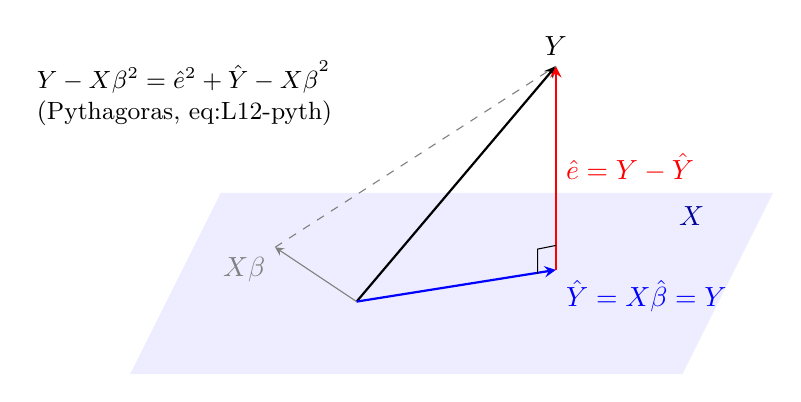
\begin{tikzpicture}[scale=1.15,>=stealth]
\fill[blue!7] (-2.5,-0.8) -- (3.6,-0.8) -- (4.6,1.2) -- (-1.5,1.2) -- cycle;
\node[blue!60!black] at (3.7,0.95) {$\colsp{X}$};
\coordinate (O) at (0,0);
\coordinate (P) at (2.2,0.35);
\coordinate (Y) at (2.2,2.6);
\coordinate (Q) at (-0.9,0.6);
\draw[->,thick] (O) -- (Y) node[above] {$Y$};
\draw[->,thick,blue] (O) -- (P) node[below right] {$\hat Y=X\hat\beta=\PX Y$};
\draw[->,thick,red] (P) -- (Y) node[midway,right] {$\hat e=Y-\hat Y$};
\draw[->,gray] (O) -- (Q) node[below left] {$X\beta$};
\draw[dashed,gray] (Q) -- (Y);
\draw (2.2,0.62) -- (2.0,0.58) -- (2.0,0.31);
\node[font=\small,align=left] at (-1.9,2.3) {$\pnorm{Y-X\beta}^2=\pnorm{\hat e}^2+\pnorm{\hat Y-X\beta}^2$\\(Pythagoras, \eqref{eq:L12-pyth})};
\end{tikzpicture}
\caption{Least squares geometry. $X\hat\beta$ is the foot of the perpendicular from $Y$ to the plane $\colsp{X}$. The residual $\hat e$ is orthogonal to $\colsp{X}$ (the normal equations), and every other $X\beta$ is farther from $Y$.}
\label{fig:L12-geometry}
\end{figure}

The name ``normal'' refers to this picture: the residual is \emph{normal} (perpendicular) to the
column space.

\begin{example}[Simple linear regression in matrix form]\label{ex:L12-slr}
Take $x=(1,2,3,4)$, $Y=(2,3,5,6)\T$ and $X=[\one,x]$ as in \cref{ex:L09-slr}. Then
\[
X\T X=\begin{pmatrix}4&10\\10&30\end{pmatrix},\qquad X\T Y=\begin{pmatrix}16\\47\end{pmatrix},\qquad
\det(X\T X)=120-100=20 .
\]
So
\[
\hat\beta=(X\T X)^{-1}X\T Y=\frac1{20}\begin{pmatrix}30&-10\\-10&4\end{pmatrix}\begin{pmatrix}16\\47\end{pmatrix}
=\frac1{20}\begin{pmatrix}480-470\\-160+188\end{pmatrix}=\begin{pmatrix}0.5\\1.4\end{pmatrix},
\]
exactly as in \cref{ex:L05-hand}, with $R_0^2=0.2$. Written out, the two normal equations
are $\sum_i\hat e_i=0$ and $\sum_ix_i\hat e_i=0$ (\cref{cor:L05-props}).
\end{example}

\begin{example}[A rank-deficient model: many solutions]\label{ex:L12-oneway}
One-way model, $k=2$, $n_1=n_2=2$, $\beta=(\mu,\mu_1,\mu_2)\T$ and data $Y=(3,5,8,10)\T$. With $X$ from
\cref{ex:L10-oneway}:
\[
X\T X=\begin{pmatrix}4&2&2\\2&2&0\\2&0&2\end{pmatrix},\qquad X\T Y=\begin{pmatrix}26\\8\\18\end{pmatrix}.
\]
The normal equations are $4\mu+2\mu_1+2\mu_2=26$, $2\mu+2\mu_1=8$, $2\mu+2\mu_2=18$. The first is the sum of the other
two, so they reduce to $\mu+\mu_1=4$ and $\mu+\mu_2=9$. The solution set is the line
\[
\hat\beta(t)=(t,\ 4-t,\ 9-t)\T,\qquad t\in\RR .
\]
Every $\hat\beta(t)$ gives the same fitted vector $X\hat\beta(t)=(4,4,9,9)\T$ (the group means), the same
residuals $(-1,1,-1,1)\T$, and $R_0^2=4$. The solution with the smallest norm minimises
$t^2+(4-t)^2+(9-t)^2$. Setting the derivative to zero gives $3t=13$, so $t=13/3$ and
$\hat\beta=(13/3,-1/3,14/3)\T$. This is the solution returned by the Moore--Penrose inverse (below).
\end{example}

\begin{note}[Supplementary: solutions via a generalized inverse]
A \vocab{generalized inverse} of a matrix $A$ is any matrix $\ginv A$ with $A\ginv AA=A$. Every matrix has one; the
Moore--Penrose inverse $A^{+}$ (\texttt{numpy.linalg.pinv}) is a particular choice. Then
\[
\hat\beta=\ginv{(X\T X)}X\T Y
\]
solves the normal equations. By \cref{lem:L12-colspace}, $X\T Y=X\T Xb$ for some $b$, so
$X\T X\,\ginv{(X\T X)}X\T Y=X\T X\,\ginv{(X\T X)}X\T Xb=X\T Xb=X\T Y$. With $A^{+}$ one gets the minimum-norm
solution of \cref{ex:L12-oneway}.
\end{note}

\subsection{Computation}
\nb{week04/L12\_normal\_equations.ipynb} solves the normal equations for both examples
(\texttt{numpy.linalg.solve} for full rank; \texttt{pinv} and \texttt{lstsq} for rank-deficient $X$). It
checks the Pythagorean identity \eqref{eq:L12-pyth} numerically, shows that different solutions give
the same fitted values, and compares with \texttt{statsmodels} OLS.

\subsection{Summary}
\begin{itemize}
  \item $\hat\beta$ is a least squares estimate iff it minimises $\pnorm{Y-X\beta}^2$ iff $X\T X\hat\beta=X\T Y$.
  \item Solutions always exist, because $X\T Y\in\colsp{X\T}=\colsp{X\T X}$. They are unique iff $\rank X=p$, in which case $\hat\beta=(X\T X)^{-1}X\T Y$.
  \item Pythagoras: $\pnorm{Y-X\beta}^2=\pnorm{Y-X\hat\beta}^2+\pnorm{X(\hat\beta-\beta)}^2$.
  \item The fitted values $X\hat\beta$ and the residuals are the same for every solution, and $X\T\hat e=0$.
\end{itemize}

\subsection{Exercises}
\begin{problem}\label{prob:L12-1}
Write the normal equations for $Y_i=\beta_1+\beta_2x_i+\eps_i$ in terms of $\sum x_i$, $\sum x_i^2$, $\sum Y_i$, $\sum x_iY_i$, and solve them to recover \cref{thm:L05-slr}.
\end{problem}
\begin{problem}\label{prob:L12-2}
For the one-way model with general $k$ and $n_i$, show that the normal equations reduce to $\mu+\mu_i=\bar Y_{i\cdot}$, $i=1,\dots,k$, and that $R_0^2=\SSW$.
\end{problem}
\begin{problem}\label{prob:L12-3}
Show that $\sum_i\hat e_i=0$ whenever $\one_n\in\colsp{X}$.
\end{problem}
\begin{problem}\label{prob:L12-4}
Verify that $G=\mathrm{diag}(0,\tfrac12,\tfrac12)$ is a generalized inverse of $X\T X$ in \cref{ex:L12-oneway}, and find the corresponding solution $GX\T Y$.
\end{problem}

\subsection{Further reading}
Christensen, \S2.2 (least squares estimation) and Appendix~B (generalized inverses); Rao, \S4a.2
(normal equations) and \S1b.5 (generalized inverse of a matrix).

% ============================================================
% Lecture 13 -- Theorem on least square estimates
% ============================================================
\section{A Theorem on Least Squares Estimates}\label{sec:L13}

\lectureheader{13}{XLT3vSQphCg}{Week-4 handwritten notes \texttt{Feb14.pdf}, part ``Lecture 3'' (estimable $\iff$ least squares estimate unique)}

\begin{guiding*}
By the end of this lecture you should be able to:
\begin{itemize}
  \item state and prove: $\lambda\T\beta$ is estimable if and only if its least squares estimate $\lambda\T\hat\beta$ is the same for every solution $\hat\beta$ of the normal equations;
  \item compute the least squares estimate of an estimable function in a rank-deficient model;
  \item show that the least squares estimate of an estimable function is a \emph{linear unbiased} estimate.
\end{itemize}
\end{guiding*}

\subsection{Recall}
For the linear model $(Y,X\beta,\sigma^2I_n)$ and $\lambda\in\RR^p$, the linear parametric function
$\lambda\T\beta$ is estimable if there is $\ell\in\RR^n$ with $\EE[\ell\T Y]=\lambda\T\beta$ for all $\beta$, i.e.\ if
$\ell\T Y$ is an unbiased estimate of $\lambda\T\beta$. By \cref{thm:L10-estimable} this happens iff
$\lambda\in\colsp{X\T}$. In \cref{sec:L12} we saw that the normal equations may have many solutions
(\cref{ex:L12-oneway}). So the ``least squares estimate'' $\lambda\T\hat\beta$ might depend on which solution we
pick. The theorem of this lecture says exactly when it does not.

\subsection{The theorem}
\begin{theorem}\label{thm:L13-unique}
Let $(Y,X\beta,\sigma^2I_n)$ be a linear model and $\lambda\in\RR^p$. Then $\lambda\T\beta$ is estimable if and
only if its least squares estimate is unique, i.e.\ $\lambda\T\hat\beta_1=\lambda\T\hat\beta_2$ for any two
solutions $\hat\beta_1,\hat\beta_2$ of the normal equations $X\T X\beta=X\T Y$.
\end{theorem}
\begin{proof}
($\Rightarrow$) Suppose $\lambda\T\beta$ is estimable. Then $\lambda\in\colsp{X\T}=\colsp{X\T X}$ (recall the earlier
theorem, \cref{thm:L10-estimable}, and \cref{lem:L12-colspace}). So there exists $b\in\RR^p$ with
$\lambda=X\T Xb$. Let $\hat\beta$ be any solution of the normal equations. Then
\[
\lambda\T\hat\beta=(X\T Xb)\T\hat\beta=b\T X\T X\hat\beta=b\T X\T Y ,
\]
which does not depend on the choice of $\hat\beta$. Hence the least squares estimate of $\lambda\T\beta$
is unique.

($\Leftarrow$) Suppose $\lambda\T\hat\beta$ is the same for all solutions $\hat\beta$. Take one solution $\hat\beta_1$ and any
$v\in\nullsp{X\T X}$, i.e.\ $X\T Xv=0$. Then $\hat\beta_2=\hat\beta_1+v$ is also a solution:
$X\T X\hat\beta_2=X\T X\hat\beta_1+0=X\T Y$. By assumption $\lambda\T\hat\beta_2=\lambda\T\hat\beta_1$, i.e.\ $\lambda\T v=0$. So $\lambda$ is
orthogonal to $\nullsp{X\T X}$. For the symmetric matrix $A=X\T X$,
\[
\nullsp{A}^\perp=\colsp{A\T}=\colsp{A}
\]
(the proof of \cref{prop:L10-nullspace} applied to $A$). Hence
$\lambda\in\colsp{X\T X}=\colsp{X\T}$ (\cref{lem:L12-colspace}), and $\lambda\T\beta$ is estimable by \cref{thm:L10-estimable}.
\end{proof}

\begin{note}
The set of all solutions of the normal equations is $\hat\beta_1+\nullsp{X\T X}$, and
$\nullsp{X\T X}=\nullsp{X}$ (\cref{thm:L14-colspace}). The theorem therefore says: $\lambda\T\hat\beta$ is constant on
this affine set iff $\lambda\perp\nullsp{X}$. This is the condition of \cref{prop:L10-nullspace}, now seen
from the side of the estimates rather than the side of the expectations.
\end{note}

\begin{proposition}[Least squares estimates of estimable functions are unbiased]\label{prop:L13-unbiased}
If $\lambda\T\beta$ is estimable, with $\lambda=X\T\ell$, then its least squares estimate satisfies
\[
\lambda\T\hat\beta=\ell\T X\hat\beta=\ell\T\hat Y,
\]
which is a linear function of $Y$, and $\EE[\lambda\T\hat\beta]=\lambda\T\beta$.
\end{proposition}
\begin{proof}
$\lambda\T\hat\beta=\ell\T X\hat\beta$ holds for every solution. By \cref{cor:L12-fitted}, $X\hat\beta=\hat Y$ is the same for
all solutions. In the proof of \cref{thm:L13-unique} we wrote $\lambda\T\hat\beta=b\T X\T Y$, which is linear in $Y$.
Then $\EE[b\T X\T Y]=b\T X\T X\beta=(X\T Xb)\T\beta=\lambda\T\beta$.
\end{proof}
Thus, for an estimable $\lambda\T\beta$, $\lambda\T\hat\beta$ is one of the linear unbiased estimates of \cref{sec:L10}.
Week~6 (the Gauss--Markov theorem) shows that it is the \emph{best} one.

\subsection{Examples}
\begin{example}[Continuing \cref{ex:L12-oneway}]\label{ex:L13-oneway}
The solutions are $\hat\beta(t)=(t,4-t,9-t)\T$, $t\in\RR$, and $\nullsp{X}=\mathrm{span}\{(1,-1,-1)\T\}$.
\begin{itemize}
  \item $\mu_1-\mu_2$, $\lambda=(0,1,-1)\T$: $\lambda\T\hat\beta(t)=(4-t)-(9-t)=-5$ for every $t$. It is unique, as the theorem predicts for an estimable function. The estimate is $\bar Y_{1\cdot}-\bar Y_{2\cdot}=4-9$.
  \item $\mu+\mu_2$, $\lambda=(1,0,1)\T$: $t+9-t=9=\bar Y_{2\cdot}$ for every $t$.
  \item $\mu_1$, $\lambda=(0,1,0)\T$: $\lambda\T\hat\beta(t)=4-t$ depends on $t$. It is not unique, so $\mu_1$ is not estimable.
  \item $\mu$: $\hat\mu=t$ can be any real number. With the constraint $\mu_1+\mu_2=0$ of \cref{prop:L08-constraint}, we would pick $t$ with $(4-t)+(9-t)=0$, i.e.\ $t=6.5$, so $\hat\beta=(6.5,-2.5,2.5)\T$.
\end{itemize}
\end{example}

\begin{example}[A regression design with a redundant column]\label{ex:L13-collinear}
Let $Y_i=\beta_1+\beta_2x_i+\beta_3z_i+\eps_i$ with $z_i=2x_i$ for all $i$ (for example, the same length recorded in two
units). Then $\nullsp{X}=\mathrm{span}\{(0,2,-1)\T\}$. The function $\beta_2+2\beta_3$ (the total effect of $x$) is
estimable, since $(0,1,2)\cdot(0,2,-1)=0$. The separate slopes $\beta_2$ and $\beta_3$ are not. Software fitting
this model must either drop a column or report a warning: \texttt{statsmodels} uses the
Moore--Penrose solution and flags a singular design. The notebook shows this with the data of
\cref{ex:L12-slr}.
\end{example}

\subsection{Computation}
\nb{week04/L13\_uniqueness\_of\_lse.ipynb} generates many solutions $\hat\beta+v$, $v\in\nullsp{X}$, of the
normal equations and plots $\lambda\T\hat\beta$ for estimable and non-estimable $\lambda$ (constant versus varying).
It also verifies \cref{prop:L13-unbiased} by simulation.

\subsection{Summary}
\begin{itemize}
  \item \textbf{Theorem:} $\lambda\T\beta$ is estimable $\iff$ $\lambda\T\hat\beta$ is the same for all solutions of $X\T X\beta=X\T Y$.
  \item If $\lambda=X\T Xb$, then $\lambda\T\hat\beta=b\T X\T Y$. If $\lambda=X\T\ell$, then $\lambda\T\hat\beta=\ell\T\hat Y$. It is linear in $Y$ and unbiased.
  \item Non-estimable functions (like $\mu$ or $\mu_i$ in the one-way model) have least squares ``estimates'' that depend on an arbitrary choice.
\end{itemize}

\subsection{Exercises}
\begin{problem}\label{prob:L13-1}
In the one-way model with general $k$, show that the least squares estimate of an estimable contrast $\sum_i c_i\mu_i$ ($\sum c_i=0$) is $\sum_i c_i\bar Y_{i\cdot}$.
\end{problem}
\begin{problem}\label{prob:L13-2}
Show that $\Var(\lambda\T\hat\beta)=\sigma^2\,\lambda\T\ginv{(X\T X)}\lambda$ for estimable $\lambda\T\beta$ and any generalized inverse, and that the value does not depend on the choice of $\ginv{(X\T X)}$.
\end{problem}
\begin{problem}\label{prob:L13-3}
In \cref{ex:L13-collinear}, find all solutions of the normal equations for $x=(1,2,3,4)$, $z=2x$, $Y=(2,3,5,6)\T$, and the least squares estimate of $\beta_2+2\beta_3$.
\end{problem}
\begin{problem}\label{prob:L13-4}
Give an example where $\lambda\T\hat\beta$ is the same for two particular solutions but $\lambda\T\beta$ is not estimable. Why does this not contradict the theorem?
\end{problem}

\subsection{Further reading}
Christensen, \S2.2 (Theorem 2.2.3 and the discussion of estimable functions and least squares).
Rao, \S4a.2 (least squares estimators of estimable functions are unique).

% ============================================================
% Lecture 14 -- Fundamentals of matrices
% ============================================================
\section{Fundamentals of Matrices and the Projection $P_X$}\label{sec:L14}

\lectureheader{14}{K_j3NHsQ4t8}{Week-4 handwritten notes \texttt{Feb14.pdf}, part ``Lecture 4'' (proposition on $X\beta$ and $P_X$; linear algebra review of the four subspaces, $\nullsp{A}=\nullsp{A\T A}$, rank--nullity)}

\begin{guiding*}
By the end of this lecture you should be able to:
\begin{itemize}
  \item show that $X\beta$ is estimable and that its least squares estimate is $X\hat\beta=\PX Y$, the orthogonal projection of $Y$ onto $\colsp{X}$;
  \item work with the four fundamental subspaces of a matrix, and compute them for small examples;
  \item prove $\nullsp{A}=\nullsp{A\T A}$ and $\colsp{A\T A}=\colsp{A\T}$ using the rank--nullity theorem;
  \item construct $\PX$ and list its properties.
\end{itemize}
\end{guiding*}

\subsection{Recap}
Least squares estimates are the solutions of $X\T X\beta=X\T Y$ (\cref{thm:L12-normal}). The estimate of $\lambda\T\beta$
is unique exactly when $\lambda\T\beta$ is estimable (\cref{thm:L13-unique}). Both proofs used
$\colsp{X\T X}=\colsp{X\T}$ (\cref{lem:L12-colspace}). This lecture proves it and identifies the fitted vector
geometrically.

\subsection{$X\beta$ and the orthogonal projection}
\begin{definition}[Orthogonal projection]\label{def:L14-proj}
Let $V\subseteq\RR^n$ be a subspace. A vector $w\in V$ is the \vocab{orthogonal projection} of $y\in\RR^n$ onto $V$ if
$y-w\perp V$, i.e.\ $\langle y-w,v\rangle=0$ for all $v\in V$. The matrix $P_V$ with $P_Vy=$ (projection of $y$) is the
\vocab{orthogonal projection matrix} onto $V$. For $V=\colsp{X}$ we write $\PX$.
\end{definition}

\begin{lemma}[Projection theorem]\label{lem:L14-projection}
For every subspace $V$ and every $y\in\RR^n$ the orthogonal projection $w$ exists and is unique. It is the unique
closest point of $V$ to $y$: $\pnorm{y-v}^2=\pnorm{y-w}^2+\pnorm{w-v}^2$ for all $v\in V$. The map $y\mapsto w$ is linear,
given by the matrix $P_V=\sum_{i=1}^r u_iu_i\T$ for any orthonormal basis $u_1,\dots,u_r$ of $V$. The matrix is symmetric and
idempotent ($P_V\T=P_V=P_V^2$), with $\colsp{P_V}=V$ and $\rank P_V=\tr P_V=\dim V$.
\end{lemma}
\begin{proof}
Choose an orthonormal basis $u_1,\dots,u_r$ of $V$ (Gram--Schmidt) and put $w=\sum_i(u_i\T y)u_i\in V$. For each $j$,
$u_j\T(y-w)=u_j\T y-\sum_i(u_i\T y)u_j\T u_i=u_j\T y-u_j\T y=0$. So $y-w$ is orthogonal to every basis vector, hence to $V$.
\emph{Uniqueness:} if $w,w'\in V$ both have $y-w,\ y-w'\perp V$, then $w-w'=(y-w')-(y-w)\in V\cap V^\perp$. So
$\pnorm{w-w'}^2=\langle w-w',w-w'\rangle=0$.
\emph{Closest point:} for $v\in V$, $y-v=(y-w)+(w-v)$ with $w-v\in V\perp y-w$, and expanding the square gives the
identity. \emph{Matrix:} $w=\sum_iu_i(u_i\T y)=\bigl(\sum_iu_iu_i\T\bigr)y$, so $P_V=\sum_iu_iu_i\T$. It is clearly symmetric, and
$P_V^2=\sum_{i,j}u_i(u_i\T u_j)u_j\T=\sum_iu_iu_i\T=P_V$. Its columns lie in $V$, and $P_Vu_j=u_j$, so $\colsp{P_V}=V$. Finally,
$\tr P_V=\sum_i\tr(u_iu_i\T)=\sum_iu_i\T u_i=r$.
\end{proof}

\begin{proposition}\label{prop:L14-PX}
In the linear model $(Y,X\beta,\sigma^2I_n)$, $X\beta$ is estimable (every component is), and its least squares estimate is
\[
X\hat\beta=\PX Y .
\]
\end{proposition}
\begin{proof}
$X\beta=(x_1\T\beta,\dots,x_n\T\beta)\T$, where $x_i\T$ is the $i$th row of $X$. Since $x_i=X\T e_i\in\colsp{X\T}$, every component is
estimable (\cref{thm:L10-estimable}). (The notes leave this as an exercise; $\EE[Y_i]=x_i\T\beta$ shows it directly.)
Let $\hat\beta$ solve the normal equations. By \cref{thm:L12-normal},
\[
R_0^2=\pnorm{Y-X\hat\beta}^2=\min_{\beta\in\RR^p}\pnorm{Y-X\beta}^2=\min_{v\in\colsp{X}}\pnorm{Y-v}^2 .
\]
Since $X\hat\beta\in\colsp{X}$, it is a closest point of $\colsp{X}$ to $Y$. By \cref{lem:L14-projection} the closest point is unique
and equals $\PX Y$. Hence $X\hat\beta=\PX Y$ and $R_0^2=\pnorm{Y-\PX Y}^2$.
(Alternatively: $X\hat\beta\in\colsp{X}$, and $Y-X\hat\beta\perp\colsp{X}$ because $X\T(Y-X\hat\beta)=0$; this is the definition of the projection.)
\end{proof}

\subsection{Linear algebra review: the four fundamental subspaces}
For an $m\times n$ matrix $A$ (a map $\RR^n\to\RR^m$, $x\mapsto Ax$):
\begin{itemize}
  \item \vocab{column space} $\colsp{A}=\{Ax:x\in\RR^n\}=\{b\in\RR^m:Ax=b\text{ has a solution}\}\subseteq\RR^m$;
  \item \vocab{null space} $\nullsp{A}=\{x\in\RR^n:Ax=0\}\subseteq\RR^n$;
  \item \vocab{row space} $\rowsp{A}=\colsp{A\T}\subseteq\RR^n$;
  \item \vocab{left null space} $\nullsp{A\T}\subseteq\RR^m$.
\end{itemize}
The \vocab{rank} of $A$ is $\dim\colsp{A}=\dim\rowsp{A}$ (the number of linearly independent columns, equal to the number of independent
rows). The \vocab{nullity} is $\dim\nullsp{A}$. The row space and the null space are orthogonal complements in $\RR^n$, and $\colsp{A}$ and
$\nullsp{A\T}$ are orthogonal complements in $\RR^m$.

\begin{theorem}[Rank--nullity]\label{thm:L14-ranknullity}
For an $m\times n$ matrix $A$, $\rank(A)+\dim\nullsp{A}=n$.
\end{theorem}
\begin{proof}
Let $v_1,\dots,v_s$ be a basis of $\nullsp{A}$ and extend it to a basis $v_1,\dots,v_n$ of $\RR^n$. Every $Ax$ is a combination of
$Av_{s+1},\dots,Av_n$, because $Av_1=\dots=Av_s=0$. These vectors are independent: if $A\sum_{i>s}c_iv_i=0$, then
$\sum_{i>s}c_iv_i\in\nullsp{A}=\mathrm{span}\{v_1,\dots,v_s\}$, which forces all $c_i=0$ by the independence of $v_1,\dots,v_n$. So
$\rank A=n-s$.
\end{proof}

\begin{example}[The four subspaces of a rank-one matrix]\label{ex:L14-subspaces}
The example on the board is only partly legible in the published notes. It is a $2\times 3$ matrix whose
column space is $\{b:b_2=2b_1\}$. We take
\[
A=\begin{pmatrix}1&2&1\\2&4&2\end{pmatrix}.
\]
\begin{itemize}
  \item $\colsp{A}$: every column is a multiple of $(1,2)\T$, so $\colsp{A}=\mathrm{span}\{(1,2)\T\}$. By row reduction, $Ax=b$ is solvable iff
  $R_2-2R_1$ gives $0=b_2-2b_1$, i.e.\ iff $b_2=2b_1$ (e.g.\ $b=(1,2)\T$). The rank is $1$.
  \item $\rowsp{A}=\colsp{A\T}=\mathrm{span}\{(1,2,1)\T\}$, a line in $\RR^3$.
  \item $\nullsp{A}=\{x:x_1+2x_2+x_3=0\}=\mathrm{span}\{(-2,1,0)\T,(-1,0,1)\T\}$, a plane in $\RR^3$ orthogonal to $(1,2,1)\T$.
  \item $\nullsp{A\T}=\{y:y_1+2y_2=0\}=\mathrm{span}\{(2,-1)\T\}$, orthogonal to $\colsp{A}$ in $\RR^2$.
  \item Rank--nullity: $1+2=3=n$.
\end{itemize}
\end{example}

\begin{figure}[ht]
\centering
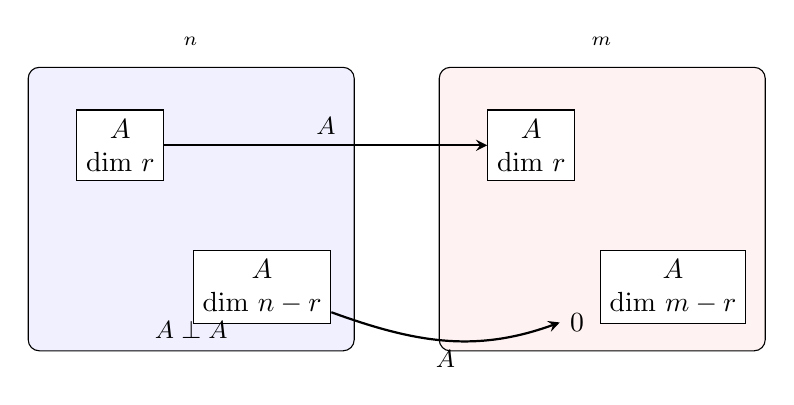
\begin{tikzpicture}[scale=0.9,>=stealth]
\draw[rounded corners,fill=blue!6] (-5.2,-1.8) rectangle (-0.6,2.2);
\node at (-2.9,2.5) {$\RR^n$};
\node[draw,fill=white,align=center] (R) at (-3.9,1.1) {$\rowsp{A}$\\dim $r$};
\node[draw,fill=white,align=center] (N) at (-1.9,-0.9) {$\nullsp{A}$\\dim $n-r$};
\draw[rounded corners,fill=red!5] (0.6,-1.8) rectangle (5.2,2.2);
\node at (2.9,2.5) {$\RR^m$};
\node[draw,fill=white,align=center] (C) at (1.9,1.1) {$\colsp{A}$\\dim $r$};
\node[draw,fill=white,align=center] (NT) at (3.9,-0.9) {$\nullsp{A\T}$\\dim $m-r$};
\draw[->,thick] (R) -- node[above,font=\small] {$A$} (C);
\draw[->,thick] (N) to[out=-20,in=-160] node[below,font=\small] {$A$} (2.3,-1.4) node[right] {$0$};
\node[font=\small] at (-2.9,-1.5) {$\rowsp{A}\perp\nullsp{A}$};
\node[font=\small] at (2.9,-1.5) {};
\end{tikzpicture}
\caption{The four fundamental subspaces. $A$ maps the row space one-to-one onto the column space and kills the null space.}
\label{fig:L14-four}
\end{figure}

\begin{theorem}\label{thm:L14-colspace}
For every $m\times n$ matrix $A$:
\begin{enumerate}
  \item $\nullsp{A}=\nullsp{A\T A}$;
  \item $\rank(A\T A)=\rank(A)$;
  \item $\colsp{A\T A}=\colsp{A\T}$.
\end{enumerate}
In particular, \cref{lem:L12-colspace} holds.
\end{theorem}
\begin{proof}
(1) If $x\in\nullsp{A}$, then $Ax=0$, so $A\T Ax=0$ and $x\in\nullsp{A\T A}$. Conversely, if $A\T Ax=0$, then
\[
0=x\T A\T Ax=\langle Ax,Ax\rangle=\pnorm{Ax}^2 ,
\]
so $Ax=0$ and $x\in\nullsp{A}$.
(2) $A$ and $A\T A$ both have $n$ columns. By rank--nullity and (1),
$\rank(A\T A)=n-\dim\nullsp{A\T A}=n-\dim\nullsp{A}=\rank(A)$.
(3) $\colsp{A\T A}\subseteq\colsp{A\T}$, because $A\T Ax=A\T(Ax)$. Both spaces have dimension $\rank(A\T A)=\rank(A)=\rank(A\T)$
by (2). A subspace contained in another of the same finite dimension equals it.
\end{proof}
\begin{note}
The notes add: ``in the recording it was mentioned $\colsp{A}$ instead of $\colsp{A\T}$''. The correct statement
is $\colsp{A\T A}=\colsp{A\T}$, a subspace of $\RR^n$. The spaces $\colsp{A\T A}$ and $\colsp{A}$ in general lie in
different spaces ($\RR^n$ versus $\RR^m$). Note also that $\colsp{AA\T}=\colsp{A}$, by the theorem applied to $A\T$.
\end{note}

\subsection{A formula for $\PX$}
\begin{proposition}[Supplementary: $\PX$ via a generalized inverse]\label{prop:L14-PXformula}
For any generalized inverse $\ginv{(X\T X)}$,
\[
\PX=X\ginv{(X\T X)}X\T ,
\]
and this matrix does not depend on the choice of generalized inverse. If $\rank X=p$, then $\PX=X(X\T X)^{-1}X\T$.
\end{proposition}
\begin{proof}
Let $G=\ginv{(X\T X)}$. By the note in \cref{sec:L12}, $\hat\beta=GX\T Y$ solves the normal equations for every $Y$. By
\cref{prop:L14-PX}, $XGX\T Y=X\hat\beta=\PX Y$ for all $Y$, so $XGX\T=\PX$. The right-hand side is the unique projection matrix, so it
does not depend on $G$.
\end{proof}

\begin{example}[$\PX$ in the one-way model]\label{ex:L14-PXoneway}
For \cref{ex:L12-oneway} ($k=2$, $n_1=n_2=2$), $\colsp{X}$ is spanned by the orthonormal vectors
$u_1=\frac1{\sqrt2}(1,1,0,0)\T$ and $u_2=\frac1{\sqrt2}(0,0,1,1)\T$. So
\[
\PX=u_1u_1\T+u_2u_2\T=\begin{pmatrix}\tfrac12&\tfrac12&0&0\\\tfrac12&\tfrac12&0&0\\0&0&\tfrac12&\tfrac12\\0&0&\tfrac12&\tfrac12\end{pmatrix},
\qquad \PX Y=\PX\begin{pmatrix}3\\5\\8\\10\end{pmatrix}=\begin{pmatrix}4\\4\\9\\9\end{pmatrix}=X\hat\beta(t)\ \ \forall t .
\]
$\tr\PX=2=\rank X$. The residual is $(I-\PX)Y=(-1,1,-1,1)\T$ and $R_0^2=4$. With $G=\mathrm{diag}(0,\tfrac12,\tfrac12)$
(\cref{prob:L12-4}), $XGX\T$ gives the same matrix.
\end{example}

\subsection{Computation}
\nb{week04/L14\_matrices\_projection.ipynb} computes the four subspaces of \cref{ex:L14-subspaces} with
\texttt{scipy.linalg.null\_space} and \texttt{orth}. It verifies $\nullsp{A}=\nullsp{A\T A}$ and the rank identities on random
rank-deficient matrices, builds $\PX$ in three ways (orthonormal basis, $X(X\T X)^{+}X\T$, $X\,\ginv{(X\T X)}X\T$ with a
hand-made $G$), and checks symmetry, idempotence and trace.

\subsection{Summary}
\begin{itemize}
  \item $X\beta$ is estimable, and its least squares estimate is $X\hat\beta=\PX Y$, the orthogonal projection of $Y$ onto $\colsp{X}$.
  \item $\PX=\sum u_iu_i\T=X\ginv{(X\T X)}X\T$: symmetric, idempotent, trace $=\rank X$.
  \item $\nullsp{A}=\nullsp{A\T A}$, $\rank A\T A=\rank A$, $\colsp{A\T A}=\colsp{A\T}$ (rank--nullity).
  \item $\rowsp{A}\perp\nullsp{A}$ in $\RR^n$ and $\colsp{A}\perp\nullsp{A\T}$ in $\RR^m$.
\end{itemize}

\subsection{Exercises}
\begin{problem}\label{prob:L14-1}
Show that $I-\PX$ is the orthogonal projection onto $\colsp{X}^\perp=\nullsp{X\T}$, and that $\PX(I-\PX)=0$.
\end{problem}
\begin{problem}\label{prob:L14-2}
Compute $\PX$ for simple linear regression with $x=(1,2,3,4)$ and verify that $\PX Y=(1.9,3.3,4.7,6.1)\T$ for $Y=(2,3,5,6)\T$.
\end{problem}
\begin{problem}\label{prob:L14-3}
For the one-way model with general $k$ and $n_i$, show that $\PX$ is block diagonal with blocks $\frac1{n_i}\one_{n_i}\one_{n_i}\T$, and that $(\PX Y)_{ij}=\bar Y_{i\cdot}$.
\end{problem}
\begin{problem}\label{prob:L14-4}
Find the four fundamental subspaces of $B=\begin{pmatrix}1&0&1\\0&1&1\end{pmatrix}$ and check rank--nullity.
\end{problem}
\begin{problem}\label{prob:L14-5}
Prove that if $P$ is symmetric and idempotent, then $P$ is the orthogonal projection onto $\colsp{P}$.
\end{problem}

\subsection{Further reading}
Christensen, Appendix~A (vector spaces), Appendix~B.3 (projections) and \S2.2; Rao, \S1a--1c (vector spaces,
matrices, projection operators) and \S4a.


\section*{Solutions to the Exercises of Chapter~\ref{ch:week04}}
\addcontentsline{toc}{section}{Solutions to the exercises}

\paragraph{\Cref{prob:L11-1}.}
With columns $(\mu,\alpha_1,\alpha_2,\beta_1,\beta_2,\beta_3)$ and cells ordered $(1,1)$, $(1,2)$, $(1,3)$, $(2,1)$, $(2,2)$, $(2,3)$:
\[
X=\begin{pmatrix}1&1&0&1&0&0\\1&1&0&0&1&0\\1&1&0&0&0&1\\1&0&1&1&0&0\\1&0&1&0&1&0\\1&0&1&0&0&1\end{pmatrix}.
\]
Column $\mu$ equals $\alpha_1+\alpha_2$ and also $\beta_1+\beta_2+\beta_3$, and by \cref{prop:L11-tworank} there is no
other relation. So $\rank X=6-2=4=I+J-1$.

\paragraph{\Cref{prob:L11-2}.}
The $\gamma_{22}$ column is zero. The non-zero cell indicators $g_{11},g_{12},g_{21}$ are independent, and all other
columns are sums of them ($\alpha_1=g_{11}+g_{12}$, $\alpha_2=g_{21}$, $\beta_1=g_{11}+g_{21}$, $\beta_2=g_{12}$). So
$\rank X=3$, the number of non-empty cells.

\paragraph{\Cref{prob:L11-3}.}
The row of $X$ for any observation in subgroup $(i,j)$ is $\lambda=e_\mu+e_{\mu_i}+e_{\delta_{ij}}$, so
$\mu+\mu_i+\delta_{ij}=\EE[Y_{ijl}]$ is estimable. Linear unbiased estimates include $Y_{ij1}$ and, better,
$\bar Y_{ij\cdot}=\frac1{n_{ij}}\sum_lY_{ijl}$.

\paragraph{\Cref{prob:L11-4}.}
The rows for cells $(1,j)$ and $(2,j)$ are $e_\mu+e_{\alpha_1}+e_{\beta_j}$ and $e_\mu+e_{\alpha_2}+e_{\beta_j}$. Their difference
is $e_{\alpha_1}-e_{\alpha_2}\in\colsp{X\T}$, so $\alpha_1-\alpha_2$ is estimable, for instance by $Y_{1j1}-Y_{2j1}$.

\paragraph{\Cref{prob:L12-1}.}
$X\T X=\begin{pmatrix}n&\sum x_i\\\sum x_i&\sum x_i^2\end{pmatrix}$ and $X\T Y=\begin{pmatrix}\sum Y_i\\\sum x_iY_i\end{pmatrix}$.
The first equation, $n\beta_1+\beta_2\sum x_i=\sum Y_i$, gives $\beta_1=\bar Y-\beta_2\bar x$. Substituting into
the second: $\beta_2(\sum x_i^2-n\bar x^2)=\sum x_iY_i-n\bar x\bar Y$, i.e.\ $\beta_2S_{xx}=S_{xY}$, which is
\cref{thm:L05-slr}.

\paragraph{\Cref{prob:L12-2}.}
$(X\T Y)_\mu=\sum_{i,j}Y_{ij}$ and $(X\T Y)_{\mu_i}=\sum_jY_{ij}=n_i\bar Y_{i\cdot}$. $(X\T X\beta)_{\mu_i}=n_i(\mu+\mu_i)$, and
$(X\T X\beta)_\mu=\sum_in_i(\mu+\mu_i)$. The $\mu_i$-equations say $\mu+\mu_i=\bar Y_{i\cdot}$. The $\mu$-equation is their
weighted sum, so it adds nothing. Then $X\hat\beta$ has entry $\bar Y_{i\cdot}$ in every row of group $i$, and
$R_0^2=\sum_{i,j}(Y_{ij}-\bar Y_{i\cdot})^2=\SSW$.

\paragraph{\Cref{prob:L12-3}.}
If $\one=Xc$, then $\one\T\hat e=c\T X\T\hat e=0$ by the normal equations.

\paragraph{\Cref{prob:L12-4}.}
$X\T XG=\begin{pmatrix}0&1&1\\0&1&0\\0&0&1\end{pmatrix}$, and multiplying by $X\T X$ gives back
$\begin{pmatrix}4&2&2\\2&2&0\\2&0&2\end{pmatrix}$. So $G$ is a generalized inverse. $GX\T Y=(0,\,8/2,\,18/2)\T=(0,4,9)\T$, which is
the solution with $t=0$.

\paragraph{\Cref{prob:L13-1}.}
By \cref{prob:L12-2} every solution has $\hat\mu+\hat\mu_i=\bar Y_{i\cdot}$. Hence
$\sum c_i\hat\mu_i=\sum c_i(\bar Y_{i\cdot}-\hat\mu)=\sum c_i\bar Y_{i\cdot}-\hat\mu\sum c_i=\sum c_i\bar Y_{i\cdot}$.

\paragraph{\Cref{prob:L13-2}.}
Write $\lambda=X\T Xb$. Then $\lambda\T\hat\beta=b\T X\T Y$ and
$\Var(\lambda\T\hat\beta)=\sigma^2b\T X\T Xb$ (\cref{prop:L09-rules}). For any generalized inverse $G$,
$\lambda\T G\lambda=b\T X\T X\,G\,X\T Xb=b\T X\T Xb$. So $\Var(\lambda\T\hat\beta)=\sigma^2\lambda\T G\lambda$, whatever $G$ is.

\paragraph{\Cref{prob:L13-3}.}
$X=[\one,x,2x]$ has $\colsp{X}=\colsp{[\one,x]}$, so the fitted values are those of \cref{ex:L12-slr}. The normal equations
reduce to $\beta_1=0.5$ and $\beta_2+2\beta_3=1.4$. All solutions are $(0.5,\ 1.4-2s,\ s)\T$, $s\in\RR$. The
estimate of the estimable function $\beta_2+2\beta_3$ is $1.4$ for every $s$.

\paragraph{\Cref{prob:L13-4}.}
Take $X=[x,x,x]$ with $x=(1,2)\T$. Then $\nullsp{X}=\{v:v_1+v_2+v_3=0\}$ is two-dimensional. For
$\lambda=(1,0,0)\T$ (not estimable, since $\lambda\T(1,-1,0)\T\ne0$), the two solutions $\hat\beta$ and $\hat\beta+(0,1,-1)\T$ give
the same $\lambda\T\hat\beta$. This does not contradict the theorem, which requires equality for \emph{all} solutions, i.e.\
$\lambda\perp$ \emph{every} $v\in\nullsp{X}$.

\paragraph{\Cref{prob:L14-1}.}
$I-\PX$ is symmetric, and $(I-\PX)^2=I-2\PX+\PX^2=I-\PX$. For $y$, $(I-\PX)y=y-\PX y\perp\colsp{X}$. Also
$y-(I-\PX)y=\PX y\in\colsp{X}$, which is orthogonal to $\colsp{X}^\perp$. By uniqueness in \cref{lem:L14-projection},
$I-\PX$ projects onto $\colsp{X}^\perp$. This space equals $\nullsp{X\T}$, because $X\T z=0$ iff $z$ is orthogonal to every
column. Finally $\PX(I-\PX)=\PX-\PX^2=0$.

\paragraph{\Cref{prob:L14-2}.}
$(X\T X)^{-1}=\frac1{20}\begin{pmatrix}30&-10\\-10&4\end{pmatrix}$, so $(\PX)_{ij}=\frac1{20}(30-10(x_i+x_j)+4x_ix_j)$:
\[
\PX=\begin{pmatrix}0.7&0.4&0.1&-0.2\\0.4&0.3&0.2&0.1\\0.1&0.2&0.3&0.4\\-0.2&0.1&0.4&0.7\end{pmatrix},
\qquad \PX(2,3,5,6)\T=(1.9,3.3,4.7,6.1)\T .
\]
The trace is $0.7+0.3+0.3+0.7=2=\rank X$.

\paragraph{\Cref{prob:L14-3}.}
The normalised group indicators $u_i=\one_{(i)}/\sqrt{n_i}$ form an orthonormal basis of $\colsp{X}$, where $\one_{(i)}$ is the
indicator of group $i$. They are orthogonal because their supports are disjoint. Hence
$\PX=\sum_i\frac1{n_i}\one_{(i)}\one_{(i)}\T$, which is block diagonal with blocks $\frac1{n_i}\one\one\T$. Then
$(\PX Y)_{ij}=\frac1{n_i}\sum_lY_{il}=\bar Y_{i\cdot}$.

\paragraph{\Cref{prob:L14-4}.}
$\rank B=2$, so $\colsp{B}=\RR^2$ and $\nullsp{B\T}=\{0\}$. $\rowsp{B}=\mathrm{span}\{(1,0,1)\T,(0,1,1)\T\}$ and
$\nullsp{B}=\mathrm{span}\{(1,1,-1)\T\}$, which is orthogonal to both rows. Rank--nullity: $2+1=3$.

\paragraph{\Cref{prob:L14-5}.}
For $y\in\RR^n$, $Py\in\colsp{P}$. For any $v=Pz\in\colsp{P}$,
$\langle y-Py,Pz\rangle=z\T P\T(y-Py)=z\T(Py-P^2y)=0$. So $y-Py\perp\colsp{P}$, and $Py$ is the orthogonal projection
(\cref{def:L14-proj}).
